\documentclass[10pt]{beamer}

\usetheme[progressbar=frametitle]{metropolis}
\usepackage{appendixnumberbeamer}

\usepackage{booktabs}
\usepackage[scale=2]{ccicons}

\usepackage{pgfplots}
\usepgfplotslibrary{dateplot}

\usepackage{xspace}
\newcommand{\themename}{\textbf{\textsc{metropolis}}\xspace}

\title{IDP}
\subtitle{Fixed-Point Matrix Multiplication}
% \date{\today}
\date{}
\author{Pamula Bhargav Ram\\EE16BTECH11024\\Rallabandi Rishideep Reddy\\EE16BTECH11031}
\institute{Problem statement and Implementation Strategy}
% \titlegraphic{\hfill\includegraphics[height=1.5cm]{logo.pdf}}

\begin{document}

\maketitle

\begin{frame}{Table of contents}
  \setbeamertemplate{section in toc}[sections numbered]
  \tableofcontents[hideallsubsections]
\end{frame}

\section{Introduction}

\begin{frame}[fragile]{Fixed Point Matrix Multiplication}

  The main idea of fixed point arithematic is to interpret bit words as integers coupled with a scale factor: \( \displaystyle \frac{z}{2^n} \)
  \begin{figure}
    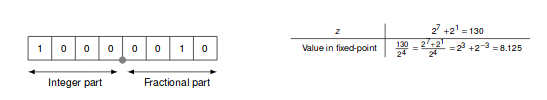
\includegraphics[scale=0.6]{Fixed.png}
  \end{figure}
  Multiplication: The product of a \(Q_{a,b}\) variable by a \(Q_{c,d}\) yields a \(Q_{a+b,c+d}\) variable.
  \begin{figure}
    {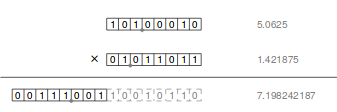
\includegraphics[scale=0.5]{MULTI.png}}
  \end{figure}
\end{frame}
\begin{frame}{Fixed Point Matrix Multiplication}
  \begin{figure}
    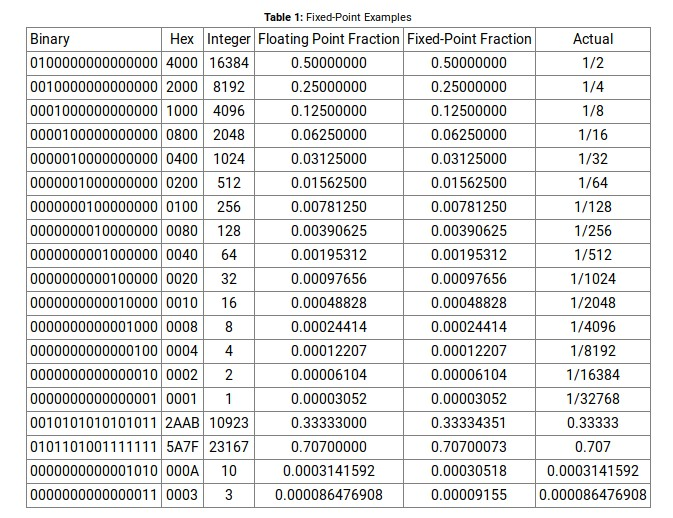
\includegraphics[scale=0.45]{Fixed_point.jpg}
  \end{figure}
\end{frame}
\begin{frame}[fragile]{Fixed Point Matrix Multiplication}
It is similar to a normal matrix multiplication. Let us recall that inner product between two vectors.
%    \begin{figure}
%        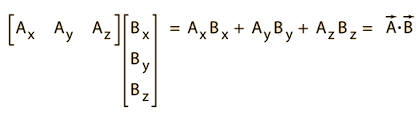
\includegraphics[scale=0.35]{vector.png}
%    \end{figure}
%    \begin{figure}
%        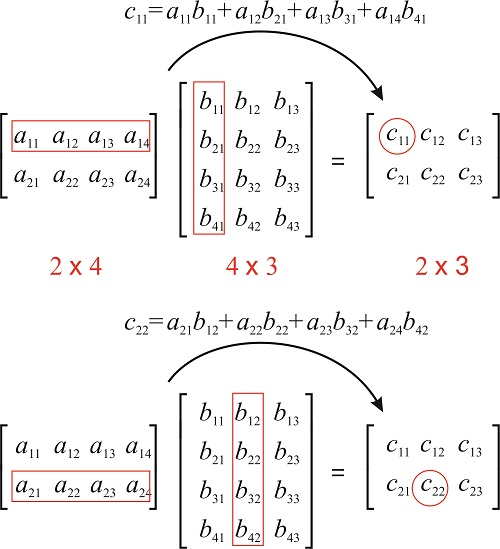
\includegraphics[scale=1]{matmul.jpg}
%    \end{figure}
  \begin{figure}
  %\centering
  % \hfill
    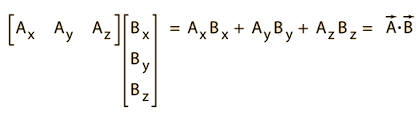
\includegraphics[scale=0.3]{vector.png}
\\From the figure it is clear that $C_{ij}$  = inner-product of $i^{th}$ row of matrix A and $j^{th}$ column of matrix B. \\
    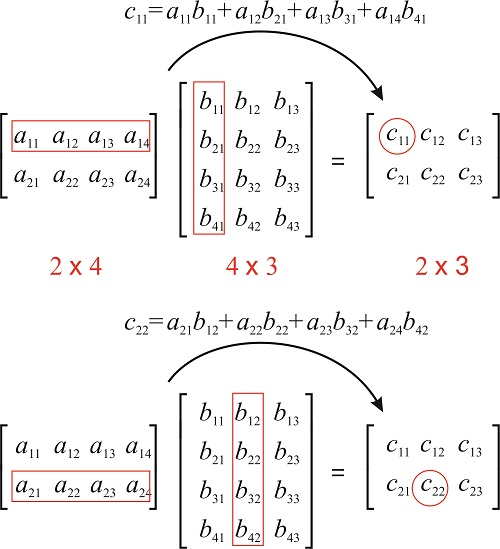
\includegraphics[scale=1]{matmul.jpg}
\end{figure}
\end{frame}


\section{Problem Statement}

\begin{frame}{Problem Statement}
	\begin{itemize}
		 \item The input is sent through Arduino and then transmitted to the icoboard whenever the clock is triggered to positive.
		 \item In order to flash verilog file in icoboard type make v\textunderscore fname = mat\textunderscore mul in terminal of RaspberryPi.
        \item Icoboard is flashed with verilog code which includes fixed point matrix multiplication logic.
        \item After executing the matrix multiplication, Icoboard outputs the matrix value to another Arduino where output is displayed.
	\end{itemize}
	
\end{frame}

\section{Implementation Strategy}

\begin{frame}[fragile]{Implementation Strategy}
	\begin{itemize}
		\item Arduino is used to input the matrix values. (i.e. matrix A and matrix B)
		\item Arduino converts floating point input to fixed point output. 
		\item Ico board receives input from Arduino where matrix multiplication is programmed.
		\item The Project will be implemented for (\(n\times n\)) matrix. And 8-bit fixed-point numbers will be used (n must be edited in the Arduino and verilog codes).
		\item For ease of demo, the implementation will be done for (\(2\times2\)) matrix.
		\item Ico board sends the output after the multiplication process to another Arduino.
		\item The output matrix can be displayed in Arduino serial monitor after floating point conversion.
	\end{itemize}
\end{frame}
\begin{frame}[fragile]{Implementation Strategy}
    \begin{itemize}
        \item whenever the input is provided at the serial monitor of the input Arduino, then a clock signal is triggered to positive edge.
        \item every time the verilog code reads positive edge from the signal coming from the Arduino, the value of the input is stored in the registers.
        \item after all the required inputs have been provided, the code stops taking inputs from Arduino. and triggers a signal for Arduino to start the matrix multiplication logic.
        \item After the matrix multiplication is over, the values are stored in the registers. 
        \item Later, when outputs are stored in registers, the code triggers another signal to the Arduino to start printing the output matrix.
        \item the output Arduino will trigger a signal for taking outputs stored in the registers at every clock signal.
    \end{itemize}
\end{frame}

\section{References}
\begin{frame}{References}
    \begin{enumerate}
        \item download and setup RaspberryPi from: \url{https://www.raspberrypi.org/downloads/raspbian/}
        \item get Arduino setup from:  \url{https://www.arduino.cc/en/Main/Software}
        \item Prorject codes are available in: \url{https://github.com/BhargavasRamus/IDP_FPGA_Spring19/tree/master/codes}
    \end{enumerate}
    
\end{frame}

{\setbeamercolor{palette primary}{fg=white, bg=blue!20}
\begin{frame}[standout]
  \Huge{THANK YOU}
\end{frame}
}


\end{document}
